\section*{Общая характеристика работы}

\newcommand{\actuality}{\underline{\textbf{\actualityTXT}}}
\newcommand{\progress}{\underline{\textbf{\progressTXT}}}
\newcommand{\aim}{\underline{{\textbf\aimTXT}}}
\newcommand{\tasks}{\underline{\textbf{\tasksTXT}}}
\newcommand{\novelty}{\underline{\textbf{\noveltyTXT}}}
\newcommand{\influence}{\underline{\textbf{\influenceTXT}}}
\newcommand{\methods}{\underline{\textbf{\methodsTXT}}}
\newcommand{\defpositions}{\underline{\textbf{\defpositionsTXT}}}
\newcommand{\reliability}{\underline{\textbf{\reliabilityTXT}}}
\newcommand{\probation}{\underline{\textbf{\probationTXT}}}
\newcommand{\contribution}{\underline{\textbf{\contributionTXT}}}
\newcommand{\publications}{\underline{\textbf{\publicationsTXT}}}


{\actuality}
Построение ядерной энергетики нового типа, устойчивой к ресурсным ограничениям и предусматривающей решение проблемы обращения с радиоактивными отходами, связано с реакторами на быстрых нейтронах, обладающими размножающими свойствами. То есть, такая система, называемая двухкомпонентной ядерной энергетикой, нацелена на воспроизводство делящегося материала -- энергетического  плутония -- в реакторе на быстрых нейтронах. Однако, по оценкам \cite{andrianovaPERSPEKTIVNYETOPLIVNYEZAGRUZKI2015}, в ближайшие десятилетия, по мере становления двухкомпонентной ядерно-энергетической системы, неизбежен переходный период, когда делящиеся материалы будут повторно использоваться в топливном цикле реакторов на тепловых нейтронах, так как они составляют основную часть парка энергоблоков. Основным материалом топлива является уран, составляющий $\approx$95\% за вычетом конструкционных материалов. К тому же, оценки показывают, что регенерированный уран с содержанием $^{235}$U на уровне от $\approx$0,85\% экономически целесообразно дообогащать на изотопно-разделительном производстве \cite{NikipelovNikipelovSudby}. 

Итак, использование выделенного из отработавшего ядерного топлива (ОЯТ) регенерированного урана является основным достижимым в ближайшей перспективе направлением вовлечения регенерируемых материалов в топливный цикл энергетических реакторов. Выделенный из ОЯТ регенерированный уран может быть использован в составе топлива ВВЭР различными способами: центрифужное дообогащение для производства уранового топлива, дообогащение и включение в состав смешанного уран-плутониевого топлива типа REMIX.

Рецикл урана является сложной задачей ввиду присутствия в изотопном составе регенерата ряда четных изотопов. В первую очередь, это неприродные $^{232}$U и $^{236}$U. Присутствие первого затрудняет обращение с регенератом, как на стадии обогащения, так и на стадии производства твэлов. Влияние же второго сказывается на ухудшении размножающих свойств ядерного топлива, поскольку данный изотоп является паразитным поглотителем тепловых нейтронов. Вдобавок, в регенерате, по сравнению с природным ураном, на порядок выше содержание $^{234}$U При этом, ориентируясь на сегодняшние тенденции к увеличению длительности топливных циклов ВВЭР, которые связаны с повышением глубины выгорания топлива, следует принять во внимание вытекающий из этого рост содержания вредных четных изотопов в регенерате.

Итак, ввиду необходимости решения задачи эффективного вовлечения регенерированного урана в ядерный топливный цикл (ЯТЦ), существует потребность поиска и дальнейшей разработки каскадных схем, которые позволят решить задачу производства из регенерата свежего топлива, удовлетворяющего стандартным спецификациям.
На сегодняшний день, хоть и предложен ряд каскадов, которые могут быть полезны для этой задачи, их границы применимости могут быть недостаточны в условиях многократного рецикла.

Таким образом, учитывая принятое в ГК Росатом стратегическое решения перехода к замкнутому ЯТЦ, решение перечисленных задач представляется актуальным для современной разделительной науки. 

{\aim} диссертационной работы является изучение физических закономерностей
молекулярно-селективного массопереноса в ординарных и многопоточных каскадах
для разделения многокомпонентных смесей с целью дальнейшего поиска
оптимальных условий обогащения регенерированного урана в подобных каскадах при
его многократном использовании в различных видах регенерированного ядерного
топлива для реакторов на тепловых нейтронах.

Для~достижения поставленной цели необходимо было решить следующие {\tasks}:
\begin{enumerate}
  \item Анализ физических закономерностей массопереноса компонентов смеси
  регенерированного урана в ординарном каскаде.
  Выявление физических причин
  невозможности решения задачи обогащения регенерата произвольного изотопного
  состава в одиночном каскаде при одновременном выполнении условий на
  концентрации изотопов $^{232}$U, $^{234}$U и $^{236}$U в получаемом продукте – низкообогащенном уране, а также априорная оценка возможности или невозможности решения этой задачи.
  \item Физическое обоснование принципов построения двойных каскадов,
  позволяющих корректировать изотопный состав регенерата по концентрациям
  изотопов $^{232}$U, $^{234}$U и $^{236}$U с одновременным расходованием полного количества
  подлежащего обогащению регенерата при различных исходных концентрациях
  четных изотопов в нем.
  \item Обоснование физических принципов «утилизации» загрязненной четными
  изотопами фракции, возникающей в двойных каскадах, путем полной или
  частичной подачи данной фракции в третий каскад с предварительным
  перемешиванием ее с природным, обедненным и/или низкообогащенным ураном.
  \item Изучение физических закономерностей изменения изотопного состава регенерата и
  интегральных характеристик модифицированных двойных каскадов и тройных
  каскадов при обогащении регенерированного урана с различным исходным
  содержанием четных изотопов.
  \item Обобщение и систематизация подходов к выбору каскадной схемы, позволяющих
  эффективное обогащение регенерированного урана в условиях однократного и
  многократного рецикла.
  \item Определение физических закономерностей изменения изотопного состава
  регенерированного урана и параметров модифицированного двойного каскада для
  его дообогащения при многократном рецикле урана (отдельно и совместно с
  плутонием) в топливе реакторов типа ВВЭР.
\end{enumerate}


{\novelty}
\begin{enumerate}
  \item Впервые предложены модификации двойных каскадов, позволяющих корректировать
  изотопный состав регенерата по концентрациям изотопов $^{232}$U, $^{234}$U и $^{236}$U с одновременным расходованием полного количества подлежащего обогащению регенерата при различных исходных концентрациях четных изотопов в нем.
  \item Обоснованы физические принципы построения тройных каскадных схем для максимально полного использования использования исходного регенерированного урана для воспроизводства топлива реакторов на тепловых нейтронах.
  \item Выполнены оригинальные исследования по изучению физических закономерностей изменения изотопного состава регенерата и интегральных характеристик модифицированных двойных и тройных каскадах при обогащении регенерированного урана с различным исходным содержанием четных изотопов.
  \item Разработан обобщенный подход к выбору каскадной схемы для эффективного обогащения регенерированного урана в условиях однократного и многократного рецикла. Для этого были предложены критерии эффективности, такие как потери $^{235}$U в схеме и из регенерата, доля центрифуг, для которых превышается пороговое значение концентрации $^{232}$U, а также методы вычисления этих критериев в составных схемах.
  \item Развиты подходы оптимизации систем каскадов на основе двойного каскада: модифицированных двойных и тройных каскадов для обогащения регенерата урана по различным критериям
  эффективности, таким как:
  \begin{enumerate}
    \item расход природного урана
    \item затраты работы разделения
    \item доля потерь $^{235}$U в схеме
    \item доля потерь $^{235}$U из исходного регенерата
    \item доля ГЦ в схеме, в которых превышена предельно допустимая концентрация по $^{232}$U    
  \end{enumerate}
  \item Предложены пути утилизации высокоактивного «нештатного» отхода, образующегося в процессе обогащения регенерированного урана в двойном каскаде.
  \item Определены физические закономерности изменения изотопного состава регенерированного урана и параметров модифицированного двойного и тройного каскадов для его дообогащения при многократном рецикле урана (отдельно и совместно с плутонием) в топливе реакторов типа ВВЭР.
\end{enumerate}

{\influence} 
\begin{enumerate}
  \item Проведенный анализ физических закономерностей массопереноса компонентов смеси регенерированного урана в ординарном каскаде позволил однозначно определить условия при которых возможно/невозможно обогащение регенерированного урана различного исходного состава в одиночном каскаде.
  \item Разработанные модификации двойных и тройных каскадов позволяют эффективно решать задачу обогащения регенерированного урана с одновременным выполнением ограничений на концентрации четных изотопов и максимальным использованием исходного регенерата.
  \item Анализ результатов расчетного моделирования молекулярно-селективного массопереноса в модифицированных двойных и тройных каскадах для обогащения регенерата урана позволяет рекомендовать область практической применимости подобных схем для получения обогащенного регенерированного урана.
  \item Разработаны рекомендации по использованию результатов работы для обогащения регенерированного урана в условиях однократного и многократного рецикла в различных видах топлива.
  \item  Представленные в работе результаты могут быть использованы в расчетных группах на предприятиях и организациях, связанных как с проектированием и построением разделительных каскадов, так и непосредственным производством изотопной продукции (АО «Уральский электрохимический комбинат», АО «Сибирский химический комбинат», АО «ТВЭЛ», АО «Восточно-Европейский головной научно-исследовательский и проектный институт энергетических технологий», АО «ПО «ЭХЗ» и др.).
  \item Предложенные методики расчета могут лечь в основу технико-экономического анализа обращения с ОЯТ в части получения из восстановленного урана низкообогащенного урана, отвечающего требуемым качествам.  
  \item  Выводы работы применимы в рамках принятой ГК Росатом программы <<Сбалансированный ЯТЦ>>, нацеленной на обеспечение дополнительных конкурентных преимуществ направления зарубежных поставок ядерного топлива. Проводимое в данной работе исследование является перспективным для развития бизнеса ГК Росатом как в направлении топливных поставок, так и в обращении с облученным топливом \cite{efimenkoProblemyPerspektivyRazvitiya2017}.
  \item Разработан тренировочный программный комплекс для расчета каскада, нацеленного на возврат регенерированного урана. Код оформлен в виде лабораторной работы, которая затем внедрена в учебный процесс.
\end{enumerate}

{\methods}
Исследование проводит систематизацию научно-технической литературы, посвященной заявленной теме.
Применяются подходы, известные в современной теоретической физике, и в частности, в теории разделения изотопов в каскадах.
В ходе работы осуществляется обоснование теоретических принципов работы анализируемых каскадов, и математическое моделирование ранее не известных каскадных схем.
Для проведения расчетов использовались модельные каскады, а именно квазиидеальный каскад и его разновидность R-каскад, для которого принимается условие несмешивания пары выбранных компонентов. Рассматривался противоточный симметричный каскад ($\alpha=\beta=\sqrt{q}$).
Моделирование процессов разделения смесей изотопов урана проводилось с помощью специально разработанных специализированных компьютерных программ. Применялись современные программные средства языка программирования Julia и подключаемые библиотеки, такие как NLopt, Optim, предназначенные для решения систем нелинейных уравнений и нелинейной оптимизации, Plots.jl для визуализации результатов, и др..

{\defpositions}
\begin{enumerate}
  \item Результаты анализа физических закономерностей массопереноса компонентов смеси регенерированного урана в ординарном каскаде, позволяющие однозначно определить условия при которых возможно/невозможно обогащение регенерированного урана различного исходного состава в одиночном каскаде.
  \item Физико-математические модели, методики расчета и оптимизации модифицированных двойных и тройных каскадных схем для обогащения
  регенерата урана с одновременным выполнением условий на концентрации четных изотопов и максимальным использованием исходного материала.
  \item Методика выбора каскадной схемы обогащения регенерированного урана в условиях многократного рецикла, в зависимости от его исходного состава и принятых ограничений на концентрации четных изотопов.
\end{enumerate}
% В папке Documents можно ознакомиться в решением совета из Томского ГУ
% в~файле \verb+Def_positions.pdf+, где обоснованно даются рекомендации
% по~формулировкам защищаемых положений.

{\reliability} Надежность, достоверность и обоснованность научных положений и выводов, сделанных в диссертации, следует из корректности постановки задач, физической обоснованности применяемых приближений, использования в исследованиях методов, ранее примененных в аналогичных исследованиях, взаимной согласованности результатов исследования, а также из совпадения результатов численных экспериментов, полученных с помощью независимо разработанных методик как самим соискателем, так и другими исследователями. Корректность результатов вычислительных экспериментов гарантируется тестами и операторами проверки соответствия ограничениям, верифицирующими строгое выполнение заданных условий и соблюдение условий сходимости балансов (массовых и покомпонентных).

{\probation}
См. приложение А2.

{\contribution} Автор принимал активное участие в написании расчетных кодов, проведении вычислительных экспериментов, а также оформлении методики выбора каскадной схемы. Автором был разработан программный комплекс для сопровождения процесса принятия решений по выбору для заданной задачи каскада конфигурации, оптимальной по целевым критериям.

{\publications} 
См. приложение А1.



\section*{Содержание работы}
Во \underline{\textbf{введении}} обоснована актуальность разработки схем для обогащения регенерированного урана, вытекающая из задач долгосрочного развития ядерной энергетики, а также из существующих на сегодня ограничений ранее предложенных схем. Cформулирована цель исследования, состоящая в теоретическом обосновании эффективных способов обогащения регенерированного урана в каскадах цен­трифуг при его многократном использовании в регенерированном ядерном топливе для реакторов на тепловых нейтронах.

\underline{\textbf{Первая глава}} посвящена критическому анализу ранее предложенных каскадных схем обогащения регенерированного урана, а также краткому обзору источников по промышленному опыту обогащения регенерата урана. Проанализирована проблема четных изотопов $^{232,234,236}$U в задаче обогащения регенерированного урана с точки зрения разделительных технологий. $^{232,234}$U ухудшают радиационные характеристики ЯТ, содержание $^{232}$U в НОУ-продукте ограничено мерами радиационной безопасности персонала на разделительном и фабрикационном производстве значениями 2·10-7\% или 5·10-7\%, предельно допустимое отношение $\frac{C_{234,{P}}}{C_{235,{P}}} = 0,02$. $^{236}$U захватывает тепловые нейтроны, приводя к необходимости повышения обогащения по $^{235}$U. Раскрыто понятие многократного использования (рецикла) урана в топливе реакторов на тепловых нейтронах (рис. \ref{fig_autoref1}). При этом при реализации схемы рис. \ref{fig_autoref1} подразумевают, что при производствесвежего топлива для реактора используют весь выделенный из ОЯТ этого же реактора регенерат, что проиллюстрирована на схеме рис. \ref{fig_autoref2}. Такой подход призван обеспечить: (1) минимизацию потерь  $^{235}$U в топливном цикле; (2) максимально эффективно использовать потенциал ОЯТ для воспроизводства топлива; (3) исключить нежелательное накопление регенерата в процессе его многократного рецикла.

\begin{figure}[ht]
  \centerfloat{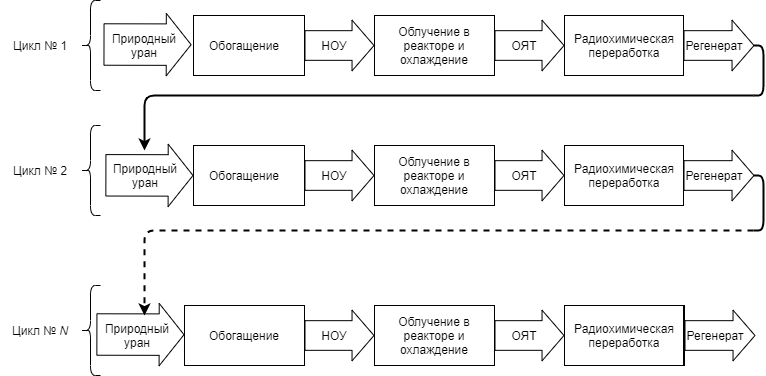
\includegraphics[scale=0.35]{theory/recycling_ru}}
  \caption{Схема многократного рециклирования урана}\label{fig_autoref1}
\end{figure}

\begin{figure}[ht]
  \centerfloat{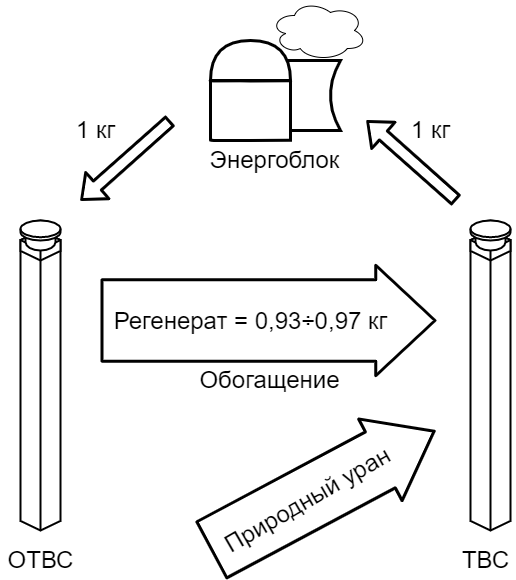
\includegraphics[scale=0.25]{cascades/ordinary/recycling1kg_ru}}
  \caption{Схема замыкания урановой топливной составляющей}\label{fig_autoref2}
\end{figure}

Приводится формулировка задачи обогащения регенерата, которой посвящена диссертационная работа: получение заданной массы товарного НОУ требуемого обогащения по $^{235}$U из сырьевого регенерата урана (в том числе многократно рециклированного) с одновременным выполнением ограничений на концентрации четных изотопов при условии расходования всей массы регенерата, выделенного из ОЯТ данного реактора. Расчёт параметров каскадной схемы, подбираемой для этой цели, подразумевает следующую математическую постановку задачи. 

Задано: 
\begin{enumerate}
  \item концентрации компонентов исходной смеси регенерированного урана -- ${C}_{i,E}, i = 232,.., 238$ (табл. \ref{is_compositions_2_5autoref});
  \item отношение потоков $E/P$ -- (исходный регенерат)/(финальный продукт);
  \item коэффициент разделения для единичной разности массовых чисел одиночного разделительного элемента -- ${q}_{0}$;
  \item концентрации $^{235}$U в потоках отбора и отвала каскада;
\end{enumerate}

\begin{table}[h]
  \centering
  \caption{{Изотопные составы регенерата различных циклов.{\label{is_compositions_2_5autoref}}}}
  \begin{tabular}{|c||c|c|c|c|c|c|}
  \hline Состав № & Массовое число & 232 & 233 & 234 & 235 & 236 \\
  \hline 1 & C, \% & $6,62\cdot10^{-7}$ & $1,19\cdot10^{-6}$ & $3,28\cdot10^{-2}$ & 1,43 & 0,9932 \\
  2 & C, \% &  $1,03\cdot10^{-6}$ & $1,3\cdot10^{-6}$ & $3,91\cdot10^{-2}$ & 1,07 & 1,45 \\\hline
  \end{tabular}
\end{table}

В процессе расчёта необходимо определить следующие параметры: 
\begin{enumerate}
  \item длины секций каскада ($N$ и $f$);
  \item концентрации остальных изотопов (кроме $^{235}$U) в выходящих потоках каскада; 
  \item отношения внешних потоков каскада к потоку питания;
  \item распределения потока и концентраций компонентов по ступеням каскада -- $L_{s}, C_{i,s} (i = 232,.., 238)$;
  \item значения срезов потоков на ступенях -- $\theta_{s}$;
  \item остальные внутренние параметры каскада ($g_{i}$, $d_{i}$, $R_{n k,F}$, $R_{n k,W}$ и $R_{n k,P}$, $\sum _{s=1}^{N}\frac{L(s)}{P}$, $\sum _{s=1}^{N}\frac{L(s)}{W}$). 
\end{enumerate}

Показана невозможность использования ординарный трехпоточный каскад \ref{ordinary} для решения сформулированной выше задачи в условиях многократного рецикла урана. Такой каскад можно использовать только для обогащения составов регенерата, в которых исходные концентрации четных изотопов меньше (на порядок или более), чем их допустимые пределы в товарном НОУ, что заведомо невыполнено при многократном рецикле урана в современных реакторов на тепловых нейтронах.

\begin{figure}[ht]
  \centerfloat{
\includegraphics[scale=0.5]{cascades/ordinary/ordinary}}
  \caption{Схема ординарного трехпоточного каскада. $F$ -- поток питания; $P$ -- поток отбора; $W$ -- поток отвала.}\label{ordinary}
\end{figure}

Проведенный анализ ранее предложенных способов обогащения регенерата, по результатам которого можно условно разделить рассмотренные способы на 3 типа: (1) схемы с разбавлением четных изотопов; (2) схемы с отделением четных изотопов; (3) «гибридные» схемы (комбинируют первые два способа).
Показано, что лишь некоторые из известных способов потенциально могут решить поставленную задачу обогащения регенерата в условиях вариьрования содержания чётных изотопов в обогащаемом регенерате. Это делает необходимым дальнейший поиск каскадных схем для решения задачи, которые можно применять для различных исходных составов регенерированного урана, а также в случаях возможного изменения внешних условий задачи. 

\underline{\textbf{Во второй главе}} приведены основные понятия и определения теории разделения изотопов в каскадах. Введение понятия  разделительного элемента, разделительной ступени, разделительного каскада и возможных вариантов соединения ступеней в каскаде. Изложены основные теоретические сведения, необходимые для моделирования разделения многокомпонентных изотопных смесей в каскадах, описаны модели «квазиидеальный» каскада как частного случая симметричного противоточного каскада, и $R$-каскада. Рассмотрены основные варианты постановок задач расчёта таких каскадов и алгоритмы их решения, которые далее используются в 3-й и 4-й главах. 

\underline{\textbf{Третья глава}} посвящена анализу причин, затрудняющих или делающих невозможным использование описанных в главе 1 способов обогащения регенерата в условиях многократного рецикла. Рассмотрены различные варианты однокаскадных схем (рис. \ref{fig:diagram1ch3}), а также двойной каскад. В качестве схем на основе ординарного каскада рассмотрены:

\begin{enumerate}
  \item схема с разбавлением природным ураном предварительно обогащенного регенерата (рис. \ref{fig:diagram1ch3}.b);
  \item схема с разбавлением предварительно обогащенного регенерата низкообогащенным ураном (рис. \ref{fig:diagram1ch3}.b);
  \item схема с разбавлением предварительно обогащенного природного урана регенератом (рис. \ref{fig:diagram1ch3}.c);
  \item схема с разбавлением регенерата природным ураном перед подачей в ординарный трехпоточный каскад (рис. \ref{fig:diagram1ch3}.a).
\end{enumerate}

Для рассмотренных схем проведена серия вычислительных экспериментов, в которых варьировали параметры каждой из схем при решении задачи обогащения регенерата, сформулированной выше. По результатам проведенных расчётов: (1) показана нецелесообразность использования схем на основе ординарных каскадов для обогащения регенерата в условиях многократного рецикла и невозможность решить задачу в большинстве случаев; (2) показана возможность обогащения регенерата с превышенными относительно допустимых пределов концентрациями четных изотопов в двойном каскаде. Однако двойной каскад позволяет только решить задачу, а именно обогатить регенерат по изотопу $^{235}$U и снизить концентрации чётных изотопов, не решая, при этом, задачи полного использования регенерата. Другой проблема, связанной с использованием двойного каскада является высокое содержание $^{236}$U в получаемом НОУ-продукте, что приводит к необходимости повышения обогащения по $^{235}$U вплоть до 6-7\% и, соответственно, росту затрат работы разделения.

\begin{figure}[ht]
  \centerfloat{\includegraphics[scale=0.47]{cascades/ord_all}}
  \caption{Схемы на основе ординарного каскада. Обозначения: $E$ -- поток питающего схему регенерата, $F_n$ -- поток разбавителя (природного урана или низкообогащенного урана); $W$ -- поток отвального ОГФУ тяжелого конца каскада; $P$ -- товарный низкообогащенный уран}\label{fig:diagram1ch3}
\end{figure}

В главе также рассмотрен двойной каскад (рис. \ref{fig:double_ru_in3}), представляющий собой последовательное соединение двух каскадов, позволяющих сконцентрировать легкие четные изотопы отдельно от изотопа $^{235}$U. Анализ проведенных расчетов обосновывает необходимость дальнейшего развития каскадных схем для решения задачи возврата регенерированного урана в ЯТЦ.

\begin{figure}[ht]
  \centerfloat{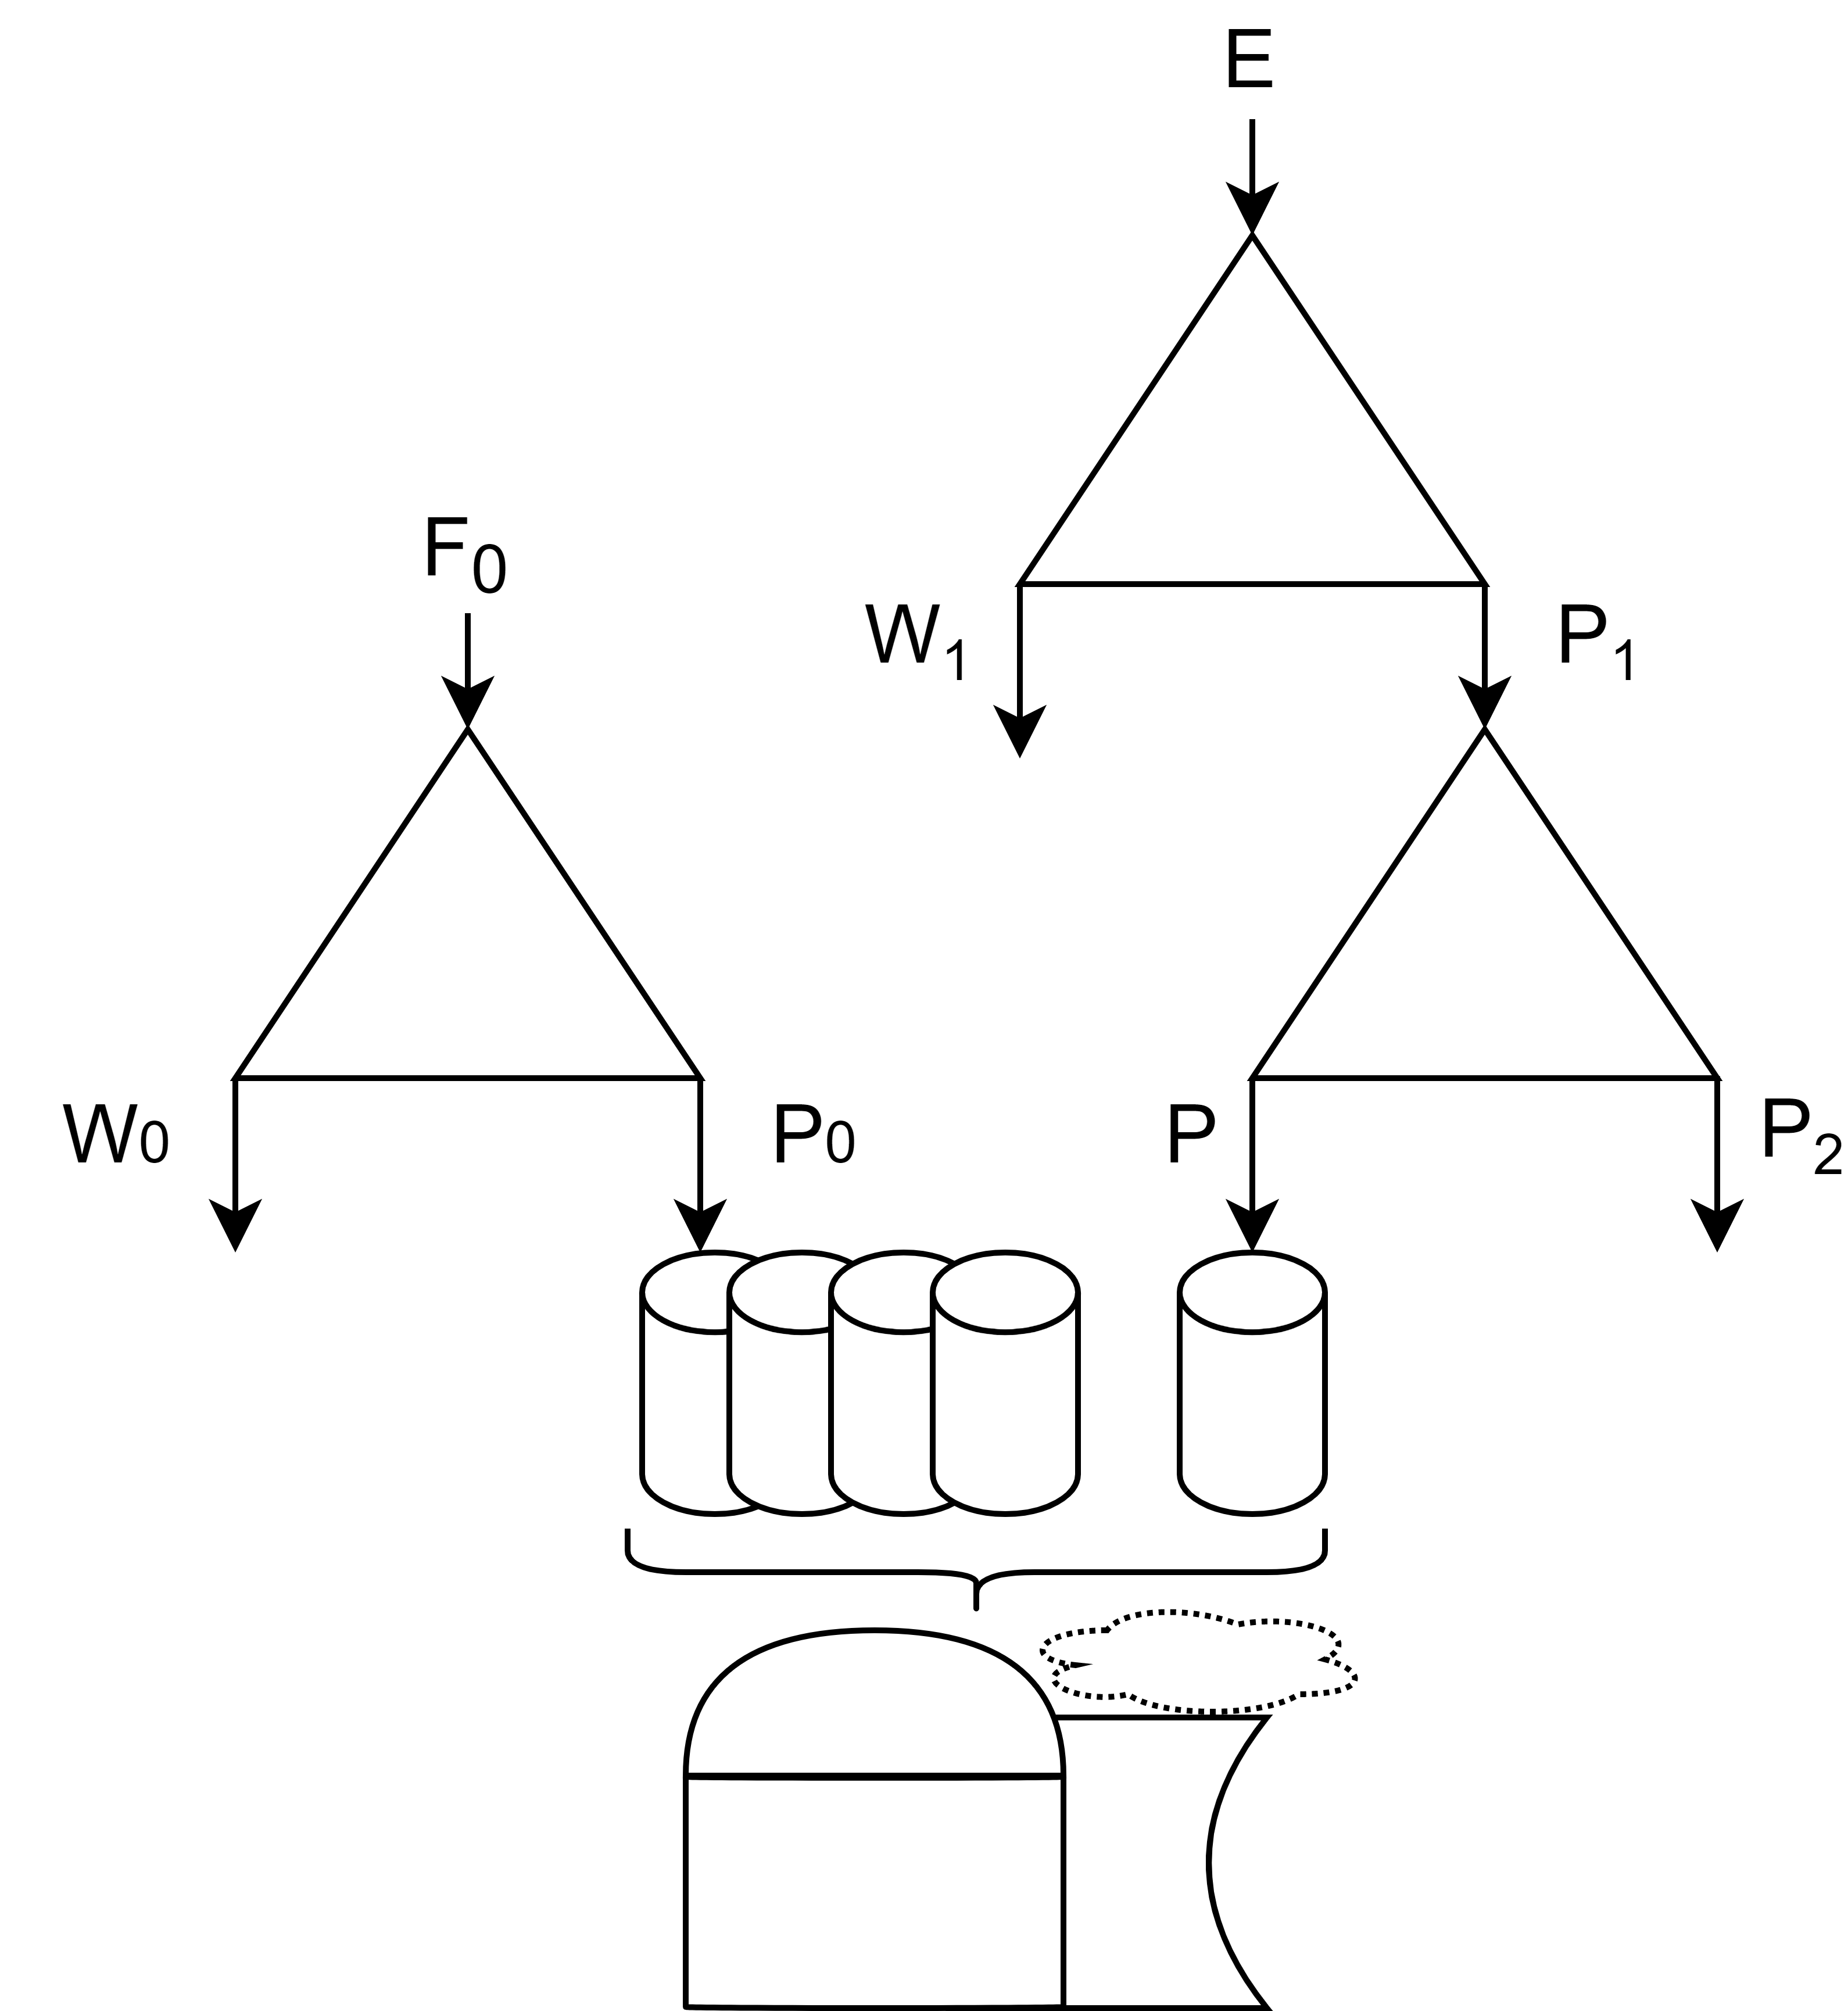
\includegraphics[scale=0.045]{cascades/Double_core}}
  \caption{Двойной каскад. Обозначения: $E$ -- поток питающего схему регенерата, $W_1$ -- поток отвального ОГФУ тяжелого конца каскада; $P$ -- конечный НОУ продукт на основе регенерата; $P_2$ -- отход двойного каскада в виде высокообогащенного урана; $F_0$ -- природный уран; $P_0$ -- дополнительно производимый НОУ продукт для возможности загрузить активную зону реактора}\label{fig:double_ru_in3}
\end{figure}


В \underline{\textbf{четвертой главе}} описаны предлагаемые в диссертации способы решения задачи обогащения регенерата в условиях его многократного рецикла.
В качестве базового предложенного способа рассмотрен <<двойной модифицированный каскад>> \ref{p2left_autoref}, который испытывается для различных исходных смесей питающего регенерата, характерных для легководного реактора. Данный способ основан на идее, изложенной в патенте АО <<СХК>> №2282904 \cite{vodolazskihSposobIzotopnogoVosstanovleniya2006}.

В каскаде I обогащают исходный регенерат изотопами $^{232,233,234,235,236}$U. В каскаде II смесь делится на две фракции, так, чтобы в потоке тяжелой фракции ($W_2$) было понижено содержание $^{232,233,234}$U по отношению к питающей второй каскад смеси -- потоку $P_1$. Затем происходит разбавление потока $W_2$ смесью, не содержащей искусственных изотопов урана для выполнения ограничений по $^{232}$U и $^{236}$U, которая нарабатывается в каскаде III.

\begin{figure}[ht]
  \centerfloat{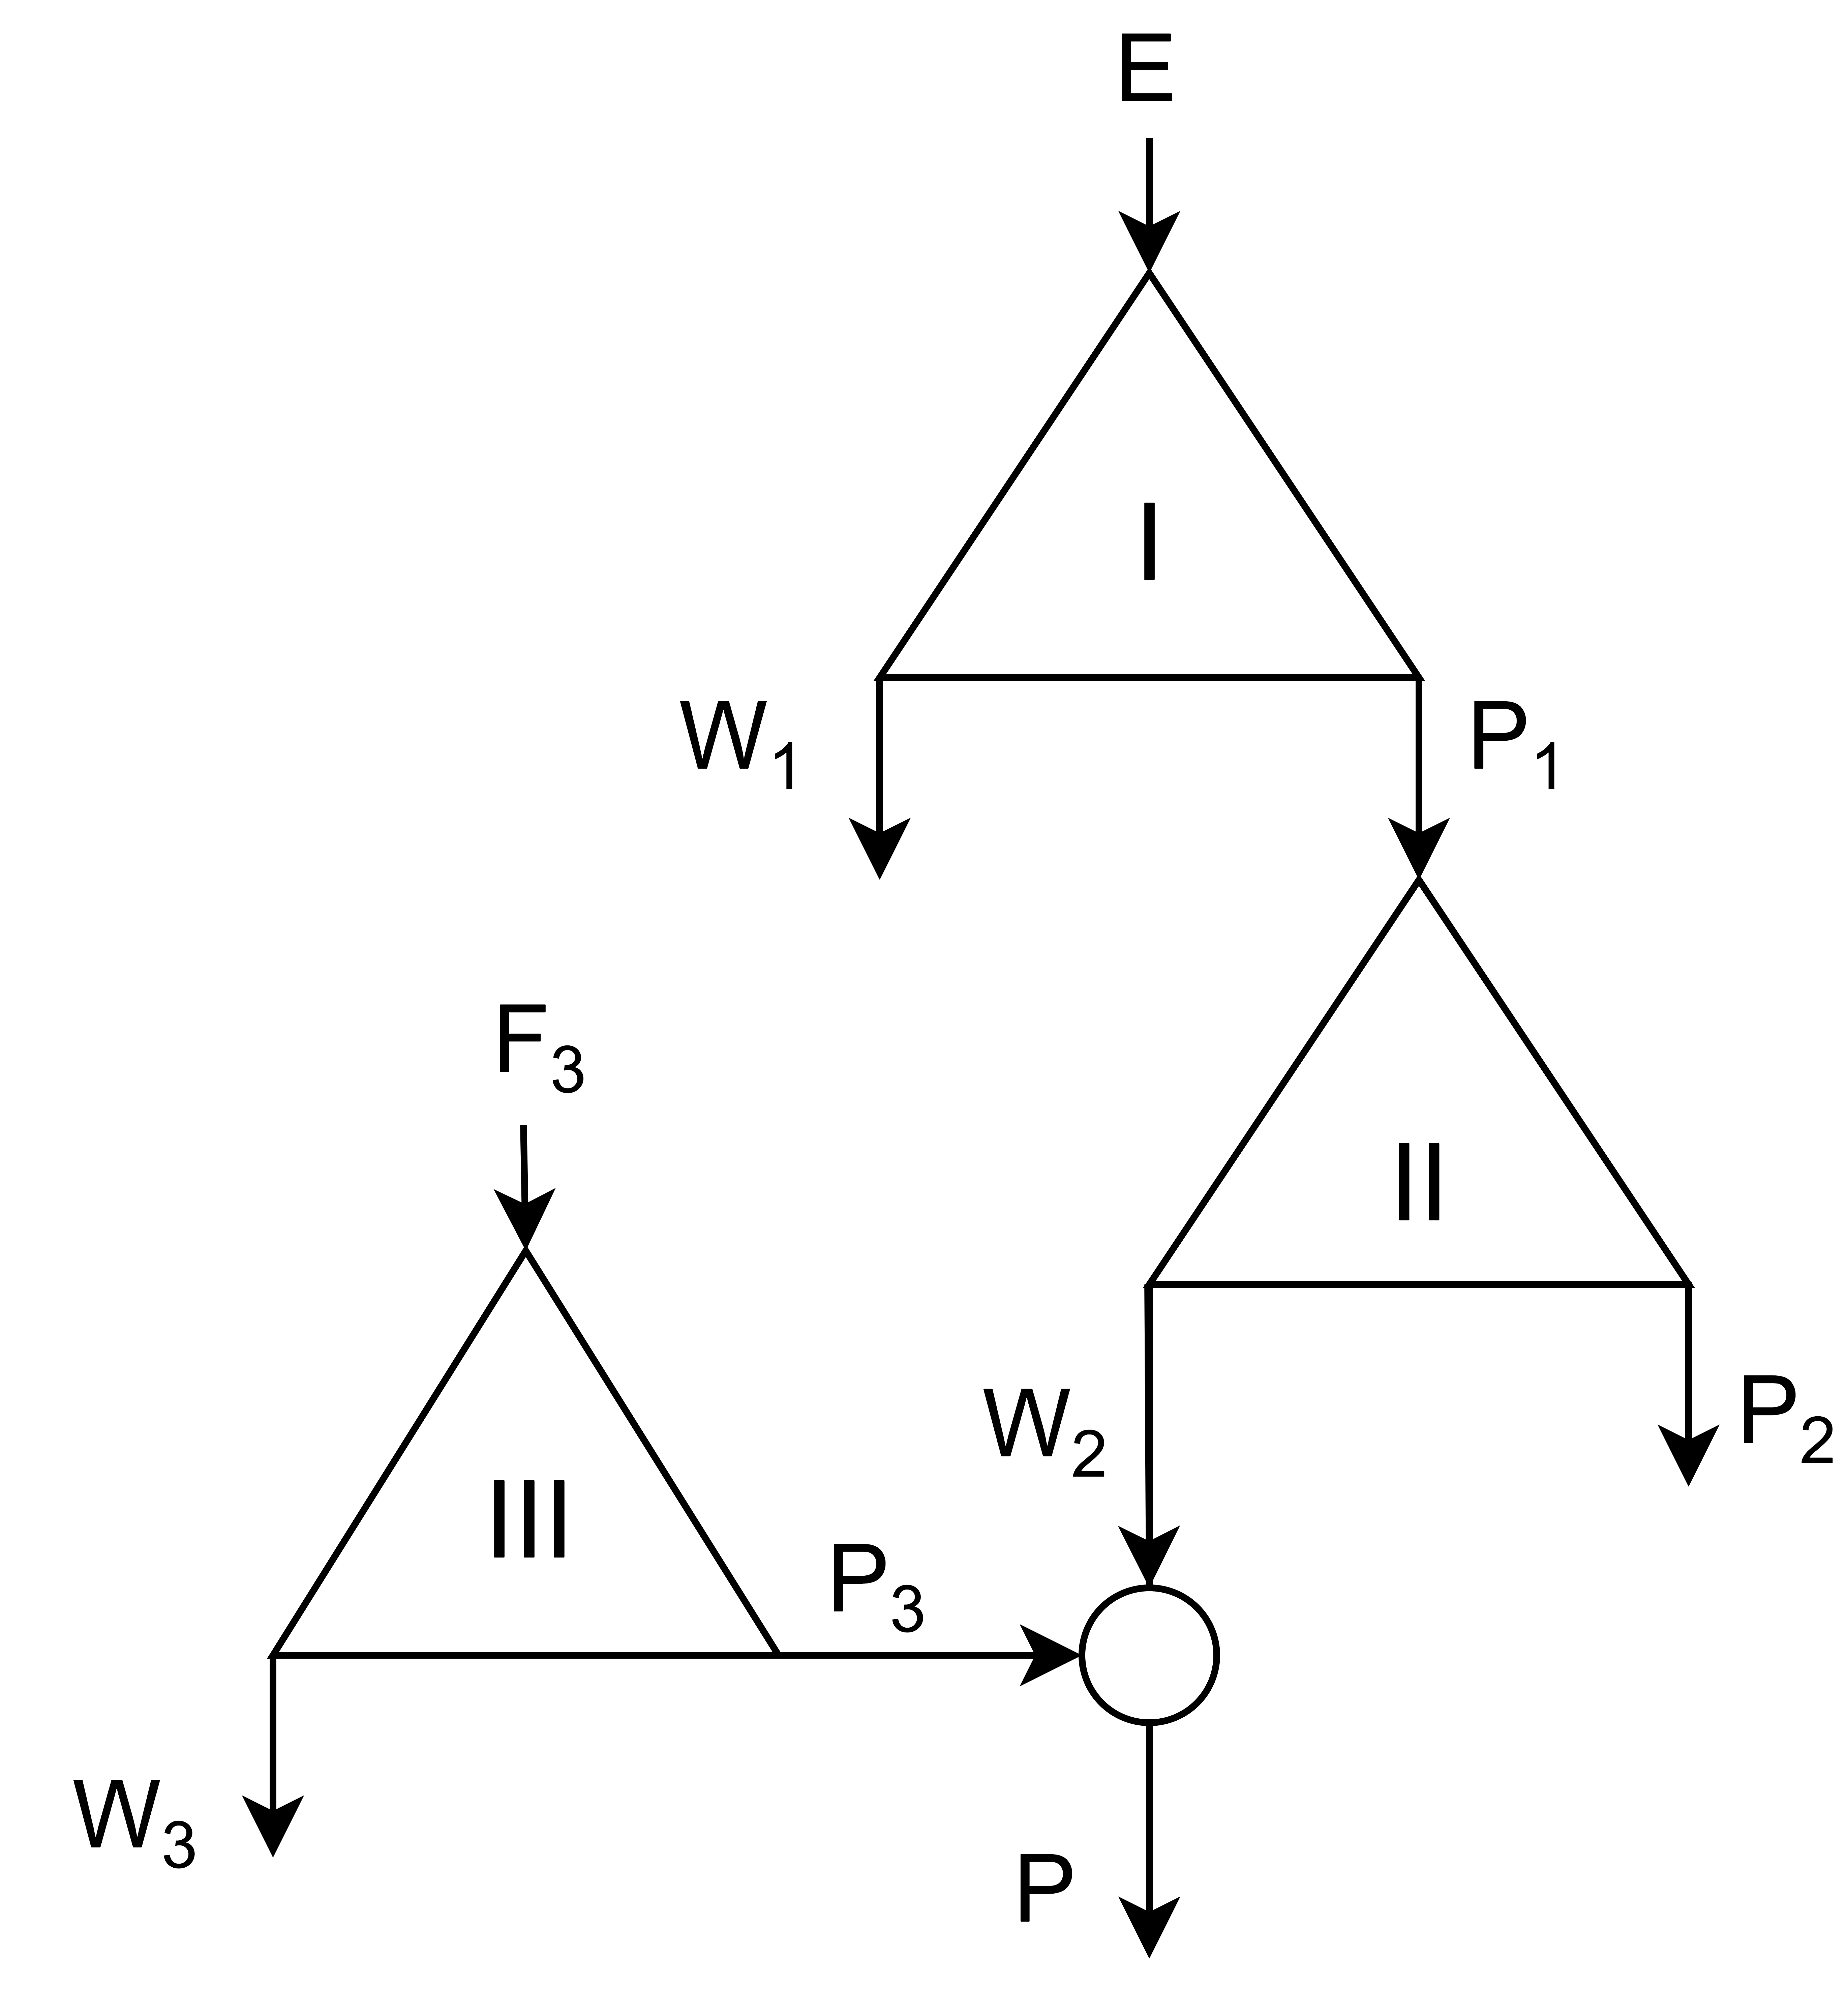
\includegraphics[scale=0.025]{cascades/DoubleModified23}}
  \caption{Схема модифицированного двойного каскада для обогащения регенерированного урана. Обозначения: $E$ -- поток регенерированного урана; $P_1$ -- поток отбора первого каскада, выступающий питанием второго каскада; $P_2$ -- поток отбора второго каскада; $W_1$ -- поток отвала первого каскада; $W_2$ -- поток тяжелой фракции (условный «отвал») второго каскада; $P_3$ -- поток НОУ-разбавителя; $P$ -- финальный продукт (товарный низкообогащенный уран (НОУ))}\label{p2left_autoref}
\end{figure}

Для схемы предложена методика расчета и оптимизации её параметров при решении задачи обогащения регенерата со всеми ограничениями. С использованием разработанной методики оценена эффективность модифицированного двойного каскада при решении задачи обогащения урана в различных условиях и при оптимизации по различным критериям эффективности. Критериями эффективности каскадной схемы выступали:

\begin{enumerate}
  \item минимум расхода природного урана ($(\delta(\frac{\Delta A}{P}))_\text{min}$);
  \item минимум затрат работы разделения ($(\delta(\frac{F_{NU}}{P}))_\text{min}$);
  \item максимум степени извлечения $^{235}$U в схеме ($(Y_f)_\text{max}$);
  \item максимум степени извлечения $^{235}$U из исходного регенерата ($(Y_{E})_\text{max}$).
\end{enumerate}  

В результате проведенных вычислительных экспериментов показано, что с использованием предложенной схемы даже для составов регенерированного урана с концентрациями четных изотопов выше предельных значений для товарного НОУ, возможно добиться экономии природного урана на уровне 15\% и выше при практически нулевом перерасходе или даже экономии затрат работы разделения. 

Сравнение оптимальных параметров модифицированного двойного каскада с аналогичными характеристиками других способов обогащения регенерата показало преимущества предложенного способа по отношению ко многим другим. Это выражается как в самом факте решения задачи, по отношению к способам, неспособным решить задачу, так и в лучших значениях расхода природного урана и затрат работы разделения по отношению к способам, решающим поставленную задачу. 

Для предложенного способа обогащения регенерата (рис. \ref{p2left_autoref}) проанализирована его «устойчивость» к изменению внешних условий таких, как:
\begin{itemize}
  \item требуемое обогащение по изотопу $^{235}$U ($C_{235,P}$);    
  \item величина предельно допустимой концентрации изотопа $^{232}$U в НОУ-продукте;
  \item расход регенерированного урана на единицу продукта ($E/P$).
\end{itemize}

Полученные результаты показали возможность решения задачи в широком диапазоне внешних условий, поскольку для всех рассмотренных комбинаций внешних параметров задачи были успешно найдены решения, т.е. подобраны параметры модифицированного двойного каскада, обеспечившие решение задачи. Таким образом, схема применима как при текущих параметрах топливного цикла и требованиях к товарному НОУ, так и потенциально может быть применена при их изменении.

В главе 4 проведено сравнение схем по ключевым характеристикам, позволяющим сопоставить экономический потенциал применения тех или иных рассмотренных схем (табл. \ref{allaut} приведена для одного из составов).
\begin{table}[ht]
  \centering
  \caption{Сравнение интегральных показателей (параметров П) схем для состава 1.{\label{allaut}}}
  \begin{tabular}{|c|c|c|c|c|c|c|}
      \hline \diagbox{П}{Схема} & $\text{1}$ & $\text{2}$ & $\text{3}$ & $\text{4}$ & $\text{5}$ & $\text{6}$\\ \hline
      $\text{$Y_{f}$}$ & 78,9 & $5,3\cdot10^{-3}$ & 40,26 & 89,0 & 89,0 & 86,9\\ \hline
      $\text{$Y_{E}$}$ & 78,9 &  48,2 &              1,0 & --    & 89,0 & 86,9\\ \hline
      $\text{$\delta(\frac{\Delta A}{P}), \%$}$ & 1,6 & 11,0 & $29,12$ & $11,0$ & 4,17 & $11,0$\\ \hline
      $\text{$\delta(\frac{F_{NU}}{P}), \%$}$ & 21,1 & 15,2 & 12,86 & $17,0$ & 6,172 & $19,0$\\ \hline
      $\text{$\frac{P_{2}}{P}$}$ & $0$ & $0$ & $0$ & $0$ & $0$ & $0,0051$\\ \hline
      $\text{$\frac{E}{P}$}$ & $4,4$ & \hl{0,76} & \hl{0,6} & \hl{0,76} & 4,71 & $0,93$\\ \hline
      $\text{$C_{232,P}, \cdot10^{-7} \%$}$ & \hl{29,0} & 5,0 & 3,97 & 5,0 & 5,0 & 5,0\\ \hline
      $\frac{C_{234,P}}{C_{235,P}}$ & \hl{0,024} & $0,011$ & 0,01085 & $0,011$ & 0,0195 & $0,012$\\ \hline
      $\text{$C_{235,P}, \%$}$ & $5,95$ & $5,10$ & $5,12$ & $5,12$ & $6,0$ & $5,1$\\ \hline
      $\text{$C_{236,P}, \%$}$ & $3,4$ & $0,51$ & 0,596 & $0,6$ & $3,6$ & $0,68$\\ \hline
      \end{tabular}   
\end{table}

Отдельно в главе 4 прорабатаны способы использования (<<утилизации>>) загрязненной легкими изотопами $^{232,234}$U фракции, получаемой в потоке $P_2$ двойного модифицированного каскада (рис. \ref{p2left_autoref}). Использование данной фракции призвано предотвратить нежелательное накопление на разделительном производстве высокоактивных отходов, а также задействовать остаточное содержание $^{235}$U в этом поке, которое может достигать 20\% и более. Предложены 3 способа и проведен их сравнительный анализ: 

\begin{itemize}
  \item Перемешивание $P_2$ с регенератом, поступающим на обогащение (рис. \ref{P2utilizationRingautoref});
  \item Получение дополнительной массы товарного НОУ (рис. \ref{P2utilizationautoref});
  \item Перемешивание $P_2$ с обедненным ураном и последующее обогащение.
\end{itemize}

\begin{figure}[ht]
  \centerfloat{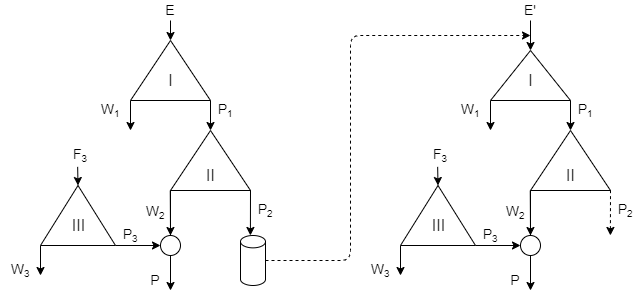
\includegraphics[scale=0.4]{cascades/P2utilizationRing}}
  \caption{Схема передачи загрязненного изотопом $^{232}$U состава гексафторида урана в двойном каскаде от первой партии дообогащенного регенерированного урана к последующей. Обозначения: $E$ -- поток регенерированного урана; $P_1$ -- поток отбора первого каскада, выступающий питанием второго каскада; $W_1$ -- поток отвала первого каскада; $W_2$ -- поток тяжелой фракции (условный «отвал») второго каскада; $P_3$ -- поток НОУ-разбавителя; $P$ -- финальный продукт (товарный низкообогащенный уран (НОУ)); $P_2$ -- поток отбора второго каскада, который подается на питание последующего двойного каскада, перемешиваясь с регенератом очередного рецикла}\label{P2utilizationRingautoref}
\end{figure}

\begin{figure}[ht]
  \centerfloat{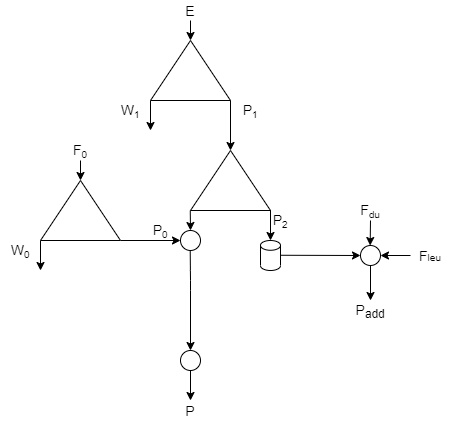
\includegraphics[scale=0.43]{cascades/P2utilization}}
  \caption{Схема независимого вовлечения в производство НОУ загрязненной изотопом $^{232}$U фракции, смешанной с обедненным и природным ураном}\label{P2utilizationautoref}
\end{figure}

Каждый из рассмотренных способов вовлечения $P_2$ в ЯТЦ демонстрирует повышение эффективности использования $^{235}$U находящегося в регенерированном уране, что позволяет получить дополнительное увеличение экономии природного урана.

Для способа утилизации легкой фракции путем ее перемешивания с регенератом, поступающим на обогащение, проведены вычислительные эксперименты по топливоподготовке (обогащение регенерата с целью производства низкообогащенного урана) для серии частичных перегрузок топлива в реакторе (замена части ТВС активной зоны реактора). Каждая из серий расчетов отличалась выбранным критерием эффективности, в качестве которых использованы $(Y_f)_\text{max}$, $(Y_{E})_\text{max}$, $(\delta(\frac{\Delta A}{P}))_\text{min}$, $(\delta(\frac{F_{NU}}{P}))_\text{min}$, $(\frac{P_2}{P})_\text{min}$. 

Для способа утилизации легкой фракции путем ее перемешивания с обедненным ураном и последующим обогащением, представленного на рис. \ref{p2_withDepU}, приводится расчетный алгоритм, с помощью которого осуществляется оценка эффективности тройного каскада по различным критериям.

\begin{figure}[ht]
  \centerfloat{\includegraphics[scale=0.02]{cascades/triple_cascade23}}
  \caption{Тройной каскад для обогащения регенерированного урана. Обозначения: $E$ -- поток регенерированного урана; $P_1$ -- поток отбора первого каскада, выступающий питанием второго каскада; $P_2$ -- поток отбора второго каскада; $F_{D}$ -- поток ОГФУ-разбавителя, смешиваемого с $P_2$ перед подачей на вход третьего каскада; $W_1$ -- поток отвала первого каскада; $W_2$ -- поток тяжелой фракции (условный «отвал») второго каскада; $P_3$ -- поток НОУ-разбавителя; $P$ -- финальный продукт (товарный низкообогащенный уран (НОУ)), полученный смешиванием потоков $W_2$, $P_3$ и $P_4$, где $P_4$ -- отбор третьего каскада; $W_4$ -- отвал третьего каскада.}\label{p2_withDepU}
\end{figure}

По результатам исследования схем, представляющих собой различные способы утилизации побочной фракции $P_2$, представлена сравнительная таблица \ref{3loopautoref}.
\begin{table}
  \centering
  \caption{Сравнение интегральных показателей схем утилизации загрязненного продукта для состава 1.{\label{3loopautoref}}}
  \renewcommand{\arraystretch}{1.2}
  \begin{tabular}{|r|c|c|c|c|c|c|c|c|c|}
    \hline
    \multirow{2}{*}{П} & \multicolumn{3}{c|}{сх. 1} & \multicolumn{3}{c|}{сх. 2} & \multicolumn{3}{c|}{сх. 3}\\
    \cline{2-10}
    & {\tiny Загр.} 1 & {\tiny Загр.} 2 & ср. & {\tiny Загр.} 1 & {\tiny Загр.} 2 & ср. & {\tiny Загр.} 1 & {\tiny Загр.} 2 & ср. \\
    \hline
    $\frac{F_{NU}}{P}$ & 6,22 & 6,49 & 6,348 & 6,21 & 6,37 & 6,29 & 6,04 & 6,04 & 6,04\\ \hline
    $\frac{\Delta A}{P}$ & 11,25 & 11,61 & 11,43 & 11,25 & 11,21 & 11,23 & 11,65 & 11,65 & 11,65 \\ \hline
    $\frac{P_2}{P}, \%$  & 1,39 & 2,96 & 2,17 & 1,39 & 1,19 & 1,29 & 0 & 0 & 0 \\ \hline
    $\frac{E}{P}$     & 0,93 & 0,95 & - & 0,93 & 0,80 & - & 0,93 & 0,93 & - \\ \hline
  \end{tabular}
\end{table}

\newpage
Выводы, относящихся ко всем рассмотренным в главе 4 схемам:
\begin{enumerate}
    \item схемы на основе двойного каскада, использующие НОУ-разбавитель, принципиально пригодны для решения задачи обогащения регенерированного урана в рамках многократного рецикла урановой составляющей топлива легководных реакторов. При этом каждая из схем имеет собственные достоинства и недостатки;
    \item характерным недостатком схемы, не предполагающей утилизацию нештатного отхода, образующегося в потоке $P_2$, является проблема с обращением с этим материалом, с высоким содержанием как четных изотопов (на 1-2 порядка выше, чем пределы для товарного НОУ) и $^{235}$U (до 20\% или, в некоторых случаях, до 90\%, в зависимости от выбранного режима работы каскадной схемы). Одним из вариантов обращения с ним, помимо схемы независимой утилизации побочного продукта легкой фракции второго каскада схемы двойного каскада с НОУ-разбавителем (рис. \ref{P2utilization}), может стать его перемешивание с отвалом первого каскада при обогащении регенерата. Оценки показали, что в этом случае возможно получить обедненный уран с приемлемым содержанием $^{232}$U (не выше $5\cdot10^{-7}$\%);
    \item характерными недостатком схемы двойного каскада с НОУ-разбавителем с возвратом потока $P_2$ в цикл (рис. \ref{P2utilizationRing}) является возврат значительной части четных изотопов на вход каскадной схемы;
    \item характерным недостатком схемы тройного каскада (рис. \ref{p2_withDepU}) являются дополнительные затраты работы разделения по отношению к схемам двойного каскада с НОУ-разбавителем, возникающие при обогащении разбавленного обедненным ураном отхода второго каскада схемы, загрязненного четными изотопами.
\end{enumerate}


\pdfbookmark{Заключение}{conclusion}                                  % Закладка pdf
В \underline{\textbf{заключении}} приведены основные выводы, сделанные в ходе диссертационного исследования и перечислены полученные результаты.

По итогу исследования выдвигаются рекомендации по использованию результатов работы для обогащения регенерированного урана в условиях однократного и многократного рецикла в различных видах топлива.

Перспективы дальнейшей разработки темы состоят в проведении технико-экономического анализа для оценки эффективности представленных схем в контексте всей цепочки ядерного топливного цикла, а также с учетом возникающих в этой цепочке изменений при использовании регенерата урана по отношению к открытому топливному циклу. Помимо этого, необходима проработка технологических проблем каждой из схем, в частности, с точки зрения возможности эксплуатации и обслуживания оборудования в условиях работы с материалами, имеющими более высокую, чем природный уран удельную активность. Например, подобные условия возникают в каскадах, концентрирующих в легкой фракции $\alpha$-активные изотопы $^{232,234}$U.

Теоретически обоснованы способы обогащения регенерированного урана с одновременной коррекцией его изотопного состава по содержанию четных изотопов, основанных на модификациях двойных каскадов. Показана применимость предложенных модификаций двойного каскада в условиях обогащения регенерированного урана с исходным содержанием четных изотопов выше допустимых пределов, что в несколько раз превышает содержание указанных изотопов в составах регенерата ранее рассмотренных в теоретических исследованиях. Это означает возможность успешного использования предложенных подходов в условиях многократного рецикла, когда концентрации четных изотопов возрастают от рецикла к рециклу.

По результатам проведенного исследования можно сформулировать следующие конкретные выводы.

\begin{enumerate}
\item В работе предложена модификация двойного каскада с НОУ-разбавителем из природного урана, применимая для обогащения регенерированного урана в условиях многократного рецикла урана в топливе легководных реакторов и позволяющая получить продукт, отвечающий всем требованиям на концентрации четных изотопов для регенерата различного исходного состава. Достоинствами схемы является возможность частичного отделения легких изотопов $^{232}$U, $^{234}$U от $^{235}$U, а также обособленность участков обогащения регенерированного урана и природного урана. Последнее обеспечивает большую вариативность в возможностях практической реализации подобной схемы, а также позволяет избежать загрязнения значительной части разделительного оборудования четными изотопами урана.


Процесс обогащения регенерата урана различного исходного состава в предложенной схеме смоделирован с использованием теории квазиидеального каскада. Разработаны оригинальные методики расчета и оптимизации предложенной каскадной схемы по различным критериям эффективности, таким как минимум расхода природного урана, минимум затрат работы разделения на получение конечного продукта, максимум степени извлечения целевого изотопа $^{235}$U из исходного регенерата и др. Проведена серия вычислительных экспериментов, позволившая оценить ключевые интегральные характеристики предложенной модификации двойного каскада (удельный расход природного урана, затраты работы разделения) в широком диапазоне изменение как ее параметров, так и внешних условий. Анализ результатов проведенных вычислительных экспериментов показал, что схема оказывается устойчивой в случаях, когда внешние ограничения <<ужесточаются>>. Например, уменьшается предельно допустимая концентрация $^{232}$U в товарном НОУ или кратно (до трех раз) возрастает масса исходного регенерированного урана, которую нужно израсходовать для получения заданной массы товарного продукта. Анализ полученных результатов создает базис для дальнейшей практической реализации подобной схемы и поиска наиболее эффективных режимов ее работы.

Анализ эффективности предложенной каскадной схемы с точки зрения потерь $^{235}$U показал, что схема позволяет извлечь более 85\% от массы $^{235}$U из исходного регенерированного урана, поступившего на обогащение. Это обеспечивает экономию природного урана по сравнению с открытым топливным циклом на уровне 15-20\% в зависимости от исходного изотопного состава регенерата. Таким образом, эта схема превышает аналогичные показатели для простейших разбавляющих схем практически вдвое.
\item Обоснован способ эффективной «утилизации» загрязненной четными изотопами фракции, возникающей в двойных каскадах при очистке от $^{232}$U, с учетом полной или частичной подачи данной фракции: а) в третий каскад с предварительным перемешиванием ее с природным, обедненным и/или низкообогащенным ураном; б) в отдельный двойной каскад, осуществляющий наработку низкообогащенного урана для последующей топливной кампании реактора. Для каждого из предложенных способов проведены вычислительные эксперименты, анализ результатов которых позволил сформулировать достоинства и недостатки каждого из способов и очертить возможные области их применения.
В качестве основных выводов по этой части приведем следующие:
\begin{enumerate}
\item Характерными недостатками схемы двойного каскада с НОУ-разбавителем с возвратом потока загрязненной $^{232}$U фракции в цикл является возврат значительной части четных изотопов на вход каскадной схемы. Это приводит к тому, что при повторении такого процесса несколько раз концентрации четных изотопов в исходном регенерате могут существенно возрастать (до нескольких раз), тем самым снижая эффективность обогащения регенерата в целом. Следовательно, такой подход применим для 1-3 таких возвратов, далее целесообразно рассмотреть возможность реализации одного из других предложенных способов утилизации отхода.
\item Характерным недостатком схемы тройного каскада для утилизации загрязненной $^{232}$U фракции является увеличение затрат работы разделения по отношению к другим рассмотренным модификациям, возникающее при обогащении разбавленного обедненным ураном загрязненного четными изотопами отхода. Анализ результатов серии вычислительных экспериментов, проведенных для данной схемы позволяет говорить, что она хорошо применима для составов регенерированного урана, когда исходное содержание $^{232}$U еще не превысило предельно допустимых значений для продукта. Иными словами, такой подход может подойти для обогащения регенерата 1-го и 2-го рецикла, позволяя вернуть в цикл более 90\% массы $^{235}$U из регенерированного урана. 
\item Схема утилизации загрязненной $^{232}$U фракции через ее разбавление обедненным ураном и НОУ из природного урана обеспечивает возможность наработки дополнительной массы отвечающего всем требованиям товарного продукта. При этом в схеме отсутствуют дополнительные каскады, что исключает дополнительные затраты работы разделения. Показано, что данный способ утилизации пригоден при обогащении различных вариантов составов исходного регенерата, что делает его перспективным в условиях многократного рецикла.
\end{enumerate}

\item Результаты работы дают основу для проведения дальнейшего технико-экономического анализа каждой из схем на основе их интегральных показателей, таких как расход природного урана, затраты работы разделения, потери $^{235}$U в цикле в контексте всей цепочки ядерного топливного цикла, а также с учетом возникающих в этой цепочке изменений при использовании регенерата урана по отношению к открытому топливному циклу. Помимо этого, необходима проработка технологических проблем каждой из схем, в частности, с точки зрения возможности эксплуатации и обслуживания оборудования в условиях работы с материалами, имеющими более высокую, чем природный уран удельную активность. 
\end{enumerate}


\insertbibliofull   
% \insertbiblioauthor
\pdfbookmark{Литература}{bibliography}
